\documentclass[]{report}
\usepackage{graphicx}
\graphicspath{{Data/}}
% Title Page
\title{Application of K-Nearest Neighbor Classification In Image Recognition}
\author{Jesse Roland}


\begin{document}
\maketitle


\begin{abstract}

	{\fontsize{14}{4}\selectfont Image recognition is an actively growing section of the Artificial Intelligence field. Numerous uses have been invented from the ability of a computer to recognize an image; such as tagging faces in photos, or allowing a robot to be aware of its surroundings. This report is being written to explain a mechanism in which a computer can learn to recognize simple gray scale images and report what they are with a high accuracy. To accomplish this, the instructor has provided images of smiles, hats, pound signs, hearts,and dollar signs. The following are samples of each:\\
	
\includegraphics{01/02}
\includegraphics{02/02}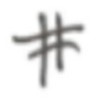
\includegraphics{03/02}
\includegraphics{04/02}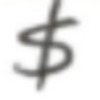
\includegraphics{05/02}
	\\There are over 70 images for each individual symbol. To accomplish image recognition, the K-Nearest Neighbor classification algorithm will be used. The training set will be 50 of each image, and the testing sets will compose 20 of each image. Accuracy will be measured by the number of correct classifications out of the total classifications.}
\end{abstract}
\section{Understanding The Concept}
{\fontsize{14}{4}\selectfont K-Nearest Neighbor is a supervised learning algorithm which featurizes training data and classifies it based on the provided labels. The algorithm then takes input and classifies it based on how close it is to already classified information. Once this is done, it will compare itself to the \textbf{k} closest other data entries, and classify the input based on the most prevalent. To better understand this concept, take the following example:\\
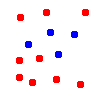
\includegraphics{knn0}\\
In the image above, some data has been input and already labeled as red or blue. Now introduce new data:\\
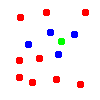
\includegraphics{knn1}\\
The green represents some inputted data, which the computer does not know the classification for. Now suppose k=4, the algorithm will then find the 4 nearest data entries to the new one:\\
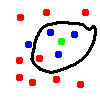
\includegraphics{knn2}\\
With three blue's and only one red, the algorithm will classify the green entry as a blue.}
\section{Application}
\subsection{Featurization}
{\fontsize{14}{4}\selectfont The first step to applying the KNN algorithm is to featurize the image so that it can be input as data. To accomplish this, an important property of the images needs to be taken into account. The instructor has stated that all images will be 100x100 pixels in size, and only use black and white. Therefore, by taking the RGB value of each pixel, one can create a set of numbers representing an image. Because all images are the same dimension, they will all be the same size as a data entry. }
\subsection{Testing}
{\fontsize{14}{4}\selectfont Due to a problem with the first image provided for a smile, images 02-51 were collected as the first 50 for training data from each symbol; resulting in a training set size of 250 images. The algorithm was then fed 20 of each symbol, images 52-72, and asked to classify each of them. Of the 100 tested, only one image of a hat was misclassified as a heart. Resulting in 99\% accuracy. 
Next, as was designated by the instructor, the program was modified to accept an image file as a parameter argument, and guess the image accordingly. The instructor stated that he will be using his own validation set, therefore all sample images provided will be fed into the algorithm. For the sake of testing, image 72 of each symbol was omitted so they could be used as valid test data for each of the following tests:\\\\
\textbf{Smile - python imageRec.py Data/01/72.jpg}\\
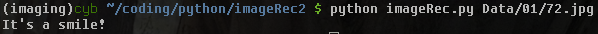
\includegraphics{test1}\\\\
\textbf{Hat - python imageRec.py Data/02/72.jpg}\\
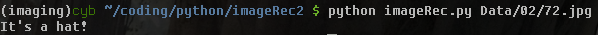
\includegraphics{test2}\\\\
\textbf{Pound Sign - python imageRec.py Data/03/72.jpg}\\
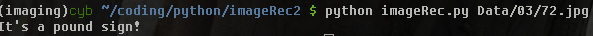
\includegraphics{test3}\\\\
\textbf{Heart - python imageRec.py Data/04/72.jpg}\\
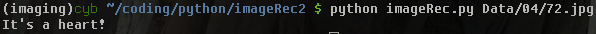
\includegraphics{test4}\\\\
\textbf{Dollar Sign - python imageRec.py Data/05/72.jpg}\\
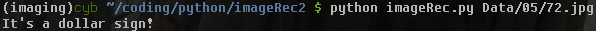
\includegraphics{test5}\\
}
\section{Conclusion}
{\fontsize{14}{4}\selectfont Overall the test provided an accuracy up to 99\%. The only misnomer that was reproduced was the mis-characterization of a hat as heart. This may be attributed to the small similarities between how the two images were drawn. Regardless of the error, this is considered to be highly accurate, correctly classifying 99/100 images. To briefly conclude; the algorithm was successful at accomplishing a high accuracy, demonstrating K-Nearest Neighbor to be an effective mechanism at image recognition.}
\end{document}          
